\documentclass{article}
\usepackage{amsmath}
\usepackage{tikz}
\usepackage{geometry}
\usepackage{enumerate}
\renewcommand{\labelenumi}{(\alph{enumi})}
\renewcommand{\labelenumii}{(\roman{enumii})}
\geometry{verbose,letterpaper,tmargin=2cm,bmargin=2cm,lmargin=2cm,rmargin=2cm}

\title{CS181: Bayesian Networks and HMMs}
\author{Danny Zhu \& Tianhui Cai}
\let\b\mathbf

\begin{document}
\maketitle

\section*{Problem 1}
\begin{center}
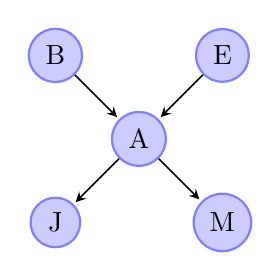
\begin{tikzpicture}[->,semithick,>=stealth,node distance=1.5cm,shorten >=1pt]
  \tikzstyle{state}=[circle,draw=blue!50,fill=blue!20,thick]
  \node [state] (B) {B};
  \node [state] (A) [below right of=B] {A};
  \node [state] (E) [above right of=A] {E};
  \node [state] (J) [below left of=A] {J};
  \node [state] (M) [below right of=A] {M};

  \path (B) edge (A)
        (E) edge (A)
        (A) edge (J)
            edge (M);
\end{tikzpicture}
\end{center}

\begin{enumerate}[(a)]
\item \textit{Let $S$ be the set of all nodes in the network. Using
  the idea of $d$-separation, for each pair of nodes $U,V\in S$, list
  the subsets of $S\setminus \{U,V\}$ that when observed would render
  $U,V$ independent.}

  \begin{tabular}{|c|c|}
  \hline
  Node pair $(U,V)$ & $S'\subset S\setminus \{U,V\},I(U,V|S')$ \\
  \hline
  $(B, A)$ & Impossible \\
  $(B, E)$ & $\emptyset$ \\
  $(B, J)$ & Any set containing $A$ \\
  $(B, M)$ & Any set containing $A$ \\
  $(E, A)$ & Impossible \\
  $(E, J)$ & Any set containing $A$ \\
  $(E, M)$ & Any set containing $A$ \\
  $(A, J)$ & Impossible \\
  $(A, M)$ & Impossible \\
  $(J, M)$ & Any set containing $A$ \\
  \hline
  \end{tabular}

\item \textit{Build another Bayesian network that has the same
  independence properties, using variable order $M,J,A,B,E$.}

  The process is to consider $M,J,A,B,E$ in order and for each node
  $N_i$ to find the minimal set of nodes $Pa(N_i)$ such that
  $P(N_i|N_1,\ldots,N_{i-1})=P(N_i|Pa(N_i))$.

  Doing this iteratively, $P(M)=P(M)$; $P(J|M)=P(J|M)$;
  $P(A|M,J)=P(A|M)$; $P(B|M,J,A)=P(B|A)$;
  $P(E|M,J,A,B)=P(E|A,B)$. Hence we get the following diagram:

  \begin{center}
    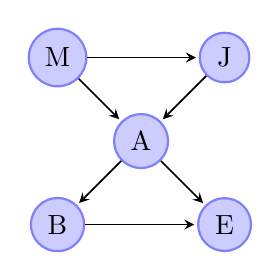
\begin{tikzpicture}[->,semithick,>=stealth,node distance=1.5cm,shorten >=1pt]
      \tikzstyle{state}=[circle,draw=blue!50,fill=blue!20,thick]
      \node [state] (B) {M};
      \node [state] (A) [below right of=B] {A};
      \node [state] (E) [above right of=A] {J};
      \node [state] (J) [below left of=A] {B};
      \node [state] (M) [below right of=A] {E};

      \path (B) edge (A)
      edge (E)
      (E) edge (A)
      (J) edge (M)
      (A) edge (J)
      edge (M);
    \end{tikzpicture}
  \end{center}
  This however doesn't actually give us all the same independence
  conditions as before: for instance, M and J are now never
  independent given any set of given nodes, whereas any set containing
  A previously would make them independent.  Hence there does not
  exist such a Bayes model with this ordering that has all the same
  independence conditions as the previous model.  This does, however,
  have the same dependence conditions as the previous model, by
  construction.
\item \textit{How many parameters are there in the BN in (a) and the
  BN in (b)?}

  (a): $1+1+4+2+2=10$.

  (b): $1+2+4+2+4=13$.

  \textit{Give three reasons why the BN in (a) is preferred over the
    BN in (b).}

  If we only care about dependence properties (which are preserved),
  \begin{enumerate}
  \item Fewer parameters means less storage.
  \item Fewer parameters means better sampling of data.
  \item No cycles $\rightarrow$ polytree $\rightarrow$ optimal
    elimination order.
  \end{enumerate}

\end{enumerate}

\section{Problem 2}
\begin{enumerate}[(a)]
\item \textit{Suppose the driver does not detect a cop and the traffic
  is slow.  Use variable elimination to determine}

  %  TODO: I'm not sure what variable elimination has to do with anything.

  \begin{enumerate}
  \item \textit{the probability of being late when the driver decides
    to speed and when the driver decides not to speed}
    \[P(OT=1|S,SC=0,ST=1) =\sum_C \sum_TP(C|SC=0)P(T|C,S)P(OT=1|T,S,ST=1)\]

    Note that by Bayes' rule,
    \[P(C=1|SC=0)=\frac{P(SC=0|C=1)P(C=1)}{P(SC=0|C=1)P(C=1)+P(SC=0|C=0)P(C=0)}=\frac{0.4\cdot 0.1}{0.4\cdot 0.1+1\cdot 0.9}=\frac{2}{47}\]
    We can rewrite
    \[P(OT=1|S,SC=0,ST=1)=\sum_T P(OT=1|T,S)g_1(T,S)\text{ where }g_1(T,S)=\sum_C P(C|SC=0)P(T|C,S)\]
    We find that $g_1(T=0,S=0)=1$, $g_1(T=1,S=0)=0$,
    $g_1(T=0,S=1)=46/47$, and $g_1(T=1,S=1)=1/47$.  Now we rewrite
    \[P(OT=1|S,SC=0,ST=1)= g_2(S)\text{ where } g_2(S)=\sum_T P(OT=1|T,S)g_1(T,S)\]
    We find that $g_2(S=0)=0.1\cdot 1$ and $g_2(S=1)=0.9\cdot
    46/47=0.88085$ so that so that the probability of being late if
    you speed is 0.11915 and the probability of being late if you
    don't speed is 0.9.

  \item \textit{the probability of getting a ticket when the driver
    decides to speed and when the driver decides not to speed}

    \[P(S|SC=0,ST=1,SC=0)=\sum_C P(T|C,S)P(C|SC=0)=g(S)\]
    Using calculations from before,

    \begin{align*}
      g(S=0)&=P(T=1|C=0,S=0)P(C=0,SC=0) + P(T=1|C=1,S=0)P(C=1|SC=0)\\
      &=0\\
      g(S=1)&=P(T=1|C=0,S=1)P(C=0,SC=0) + P(T=1|C=1,S=1)P(C=1|SC=0)\\
      &=0.5\cdot 2/47=0.021277
    \end{align*}

    so that probability of getting a ticket while speeding is 0.021277
    and probability of getting a ticket while not speeding is 0.

  \item \textit{Suppose the cost of a ticket is \$150, and the cost of
    arriving late is \$10. What is the expected utility of speeding
    and not speeding?  What would be the optimal decision?}

    Speeding: $-(150\cdot 0.021277 +10\cdot 0.11915)=-4.383$

    Not speeding: $-(150\cdot 0 +10\cdot 0.9)=-9$

    Clearly we should speed.
  \end{enumerate}

\end{enumerate}

\section*{Problem 3}
\begin{enumerate}[(a)]
  \setcounter{enumi}2
\item
  \begin{enumerate}
  \item \emph{Define the HMM for modeling the no-momentum case in terms of
    states, observations, and the model parameters necessary.}

    There are twelve states, one for each colored square on the board.

    There are four possible observations, one for each color.

    Each state can transition to any one corresponding to an adjacent
    color with probability $\frac14$, or to itself with the remaining
    probability.

    Each state leads to the observation of the corresponding color
    with probability $.925$, and to each of the other colors with
    probability $.025$.
  \item \emph{Run \emph{\texttt{viterbi.py}} on the two datasets,
    \emph{\texttt{robot\_with\_momentumdata}} and
    \emph{\texttt{robot\_no\_momentum.data}}, to learn an HMM for each
    condition and also to infer the sequences of locations visited by
    the robot. Explore when, how, and why a hidden Markov model is
    successful or not in inferring the robot's true sequences. Give a
    brief writeup of what you found; include any observations about
    how well HMMs work on these problems and why. Think of
    explanations for the observations, and for failures, think of
    modifications to lead to success.}

    \begin{itemize}
    \item \emph{What probabilistic assumptions are we making about the nature of
      the data in using a hidden Markov model?}

    \item \emph{How well do these assumptions match the actual domain?}

    \item \emph{To what extent was, or was not, performance hurt by making such
      assumptions?}

    \end{itemize}
  \end{enumerate}
\end{enumerate}
\section*{Problem 4}
\begin{enumerate}[(a)]
\item \emph{Describe the HMM for modeling this weather problem in terms of hidden
  states, observations, and the model parameters necessary.}

  There are hidden states corresponding to states of the world that we can't
  see. Observations are things like ``rain'', ``clouds'', ``sun'', ``fog'', etc. 
  The model parameters necessary are the initial probabilities of being in a
  certain state, the transition probability between states, and the probability
  of getting a particular observation given a particular states. 

\item
  \begin{enumerate}
    \setcounter{enumiii}2
  \item \emph{Use the two unit tests \emph{\texttt{test\_bw\_beta\_all\_equal}}
    and
    \emph{\texttt{test\_bw\_gamma\_first\_col\_equal}} to answer the following questions;
    include outputs in writeup.}

    \begin{enumerate}[(1)]
    \item \emph{Why are the betas all equal for each time step?}
    \item \emph{Why are the gamma values for the first state the same for all time periods?}
    \end{enumerate}

  \item \emph{Alpha and beta values get small for long sequences. If you look at the
    \emph{\texttt{get\_alpha}} function, you can see that there is normalization code.
    Why is the sum of the logs of the normalization factors the log likelihood of
    the returned observation sequence?}

    $\log(a\cdot b)=\log(a)+\log(b)$. Taking logs of small alpha and beta values
    make them less prone to encoding error.

  \end{enumerate}

\item
  \begin{enumerate}
  \item \emph{Run \texttt{\emph{classify.py}} on each data set to learn an HMM
    for each city from the training data and use them to classify the test data.
    Vary the number of hidden states from 1 to 6 and plot the final classification
    accuracy vs the number of hidden states.}

  \item \emph{Plot $\log(P(D|\Theta))$ for training the model for Boston with
    varying numbers of hidden states. Do you see any patterns?}

  \item \emph{By looking at the data and the learned models, try to explain your
    results. When do more hidden states help? When are they not needed? What is
    it about the observations that makes more states unnecessary?}

  \item \emph{The data was generated synthetically. How many hidden states do you
    think were in our generating model? Why?}

  \end{enumerate}
\end{enumerate}
\end{document}
